\chapter{Alloy modelling}

\section{Model}
\begin{minted}[tabsize=4,breaklines=true]{alloy}
open util/boolean

sig Car {
	position: one Position,
	reserved: one Bool,
	running: one Bool,
	user: one User,
	battery: one Float
} {
	battery > 0
	battery < 100
}

sig User {
	email: one String,
	name: one String,
	telephone: one String,
	resvCar: lone Car,
	drivingCar: lone Car,
	position: one Position
}

sig Position {
	latitude: one Float,
	longitude: one Float
}

sig String {}

sig PowerStation {
	carParked: set Car,
	capacity: one Int,
	position: one Position,
	amountParked: one Int
} {
	capacity > 0
	amountParked > 0
}

sig Parking {
	car: lone Car
}

fact capacityConstraint {
	all pw: PowerStation | #pw.carParked < pw.capacity
}

fact carLocationConstraint {
	all c: Car, ps:PowerStation, p: Parking | (c in ps.carParked => c != p.car) and (c = p.car => not c in ps.carParked) 
}

fact coordinatesConstraint {
	all u: User | #u.drivingCar = 1 implies u.position = u.drivingCar.position
	all c:Car, pw: PowerStation | (c in pw.carParked) implies c.position = pw.position
	all pw1, pw2 : PowerStation | pw1 != pw2 implies pw1.position != pw2.position
}

fact carConstraints {
	all c: Car | (c.running = True and #c.user = 1) implies c.user.drivingCar = c
	all c: Car | (c.reserved = True and #c.user = 1) implies c.user.resvCar = c
	all c: Car | (c.running = True implies c.reserved = False) and (c.reserved = True implies c.running = False) 
	all c: Car, ps:PowerStation, p: Parking | ((c in ps.carParked) or (c = p.car)) implies c.running = False 
	all c: Car | (c.running = True <=> #c.user.drivingCar = 1) and (c.reserved = True <=> #c.user.resvCar = 1)
}

fact userConstraints {
	all u: User | #u.drivingCar = 1 implies u.drivingCar.user = u
	all u: User | #u.resvCar = 1 implies u.resvCar.user = u
	all u: User | (#u.resvCar = 1 implies #u.drivingCar = 0) and (#u.drivingCar = 1 implies #u.resvCar = 0)
}

pred PowerStationUpdate(c,c':Car) {
	all p:PowerStation | (c in p.carParked => (one p':PowerStation | (
		p'.carParked = p.carParked - c + c' and
		p.capacity = p'.capacity and
		p.position = p'.position and
		#p.carParked = #p'.carParked)
		)
	)
}

pred UserReservesACar(c,c':Car,u,u':User) {
	#u.resvCar = 0
	#u.drivingCar = 0
	c.running = False
	c.reserved = False
	c'.running = False
	c'.reserved = True
	c'.user = u'
	c.position = c'.position
	c.battery = c'.battery
	u'.resvCar = c'
	#u.drivingCar = 0
	powerStationUpdate[c,c']
	powerStationUpdate[c',c]
}

pred UserAbortsReservation(c,c':Car,u,u':User) {
	UserReservesACar[c',c,u',u]
}

pred UserDrivesACar (c,c':Car, u,u':User) {
	c.user = u
	c'.user = u'
	c.position = c'.position
	c.battery = c'.battery
	c.reserved = True
	c'.running = True
	u.resvCar = c
	u'.drivingCar = c'
	userUnplugsACar [c]
}

pred UserUnplugsACar(c:Car) {
	all p:PowerStation | c in p.carParked => one p':PowerStation | (
		p.capacity = p'.capacity and p.position = p'.position 
		and p'.carParked = p.carParked - c and p.amountParked = plus[p'.amountParked,1])
}

pred UserFinishesARide(c,c':Car) {
	c.battery = c'.battery
	c.position = c'.position
	c.running = True
	c'.reserved = False
	c'.running = False
	UserPlugsACarIn[c']
}

pred UserPlugsACarIn(c':Car) {
	all p,p':PowerStation | p.capacity = p'.capacity and p.position = p'.position
	all p:PowerStation | p.position = c'.position and c' not in p.carParked => 
	one p':PowerStation | (p'.carParked = p.carParked + c' and p'.amountParked = plus[p.amountParked,1])
	all p:PowerStation | c' in p.carParked => one p':PowerStation | (p'.carParked = p.carParked - c'
	and p'.amountParked = minus[p.amountParked,1])
}

assert CarCanHaveOneState {
	all c:Car | not (c.reserved = True and c.running = True)
}

assert UserCanHaveOneState {
	all u:User | not (#u.drivingCar = 1 and #u.resvCar = 1)
}

run UserDrivesACar for 5
run UserFinishesARide for 5
run UserReservesACar for 5
run UserAbortsReservation for 5
check CarCanHaveOneState for 5
check UserCanHaveOneState for 5
\end{minted}

\section{Alloy result}
\begin{figure}[h]
	\centering
	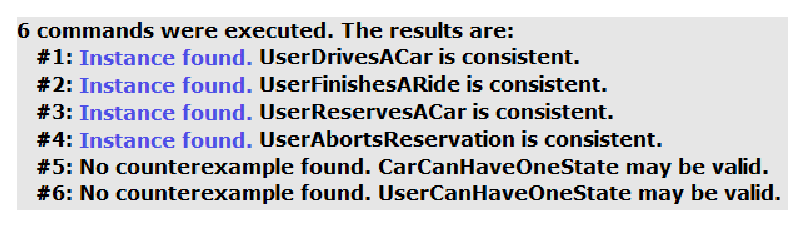
\includegraphics[width=\linewidth,keepaspectratio]{figures/alloy_results.eps}
	\caption{Alloy result of the model}
	\label{fig:alloy_results}
\end{figure}

\clearpage
\section{World generated}

\subsection{UserDrivesACar}
\begin{figure}[h]
	\centering
	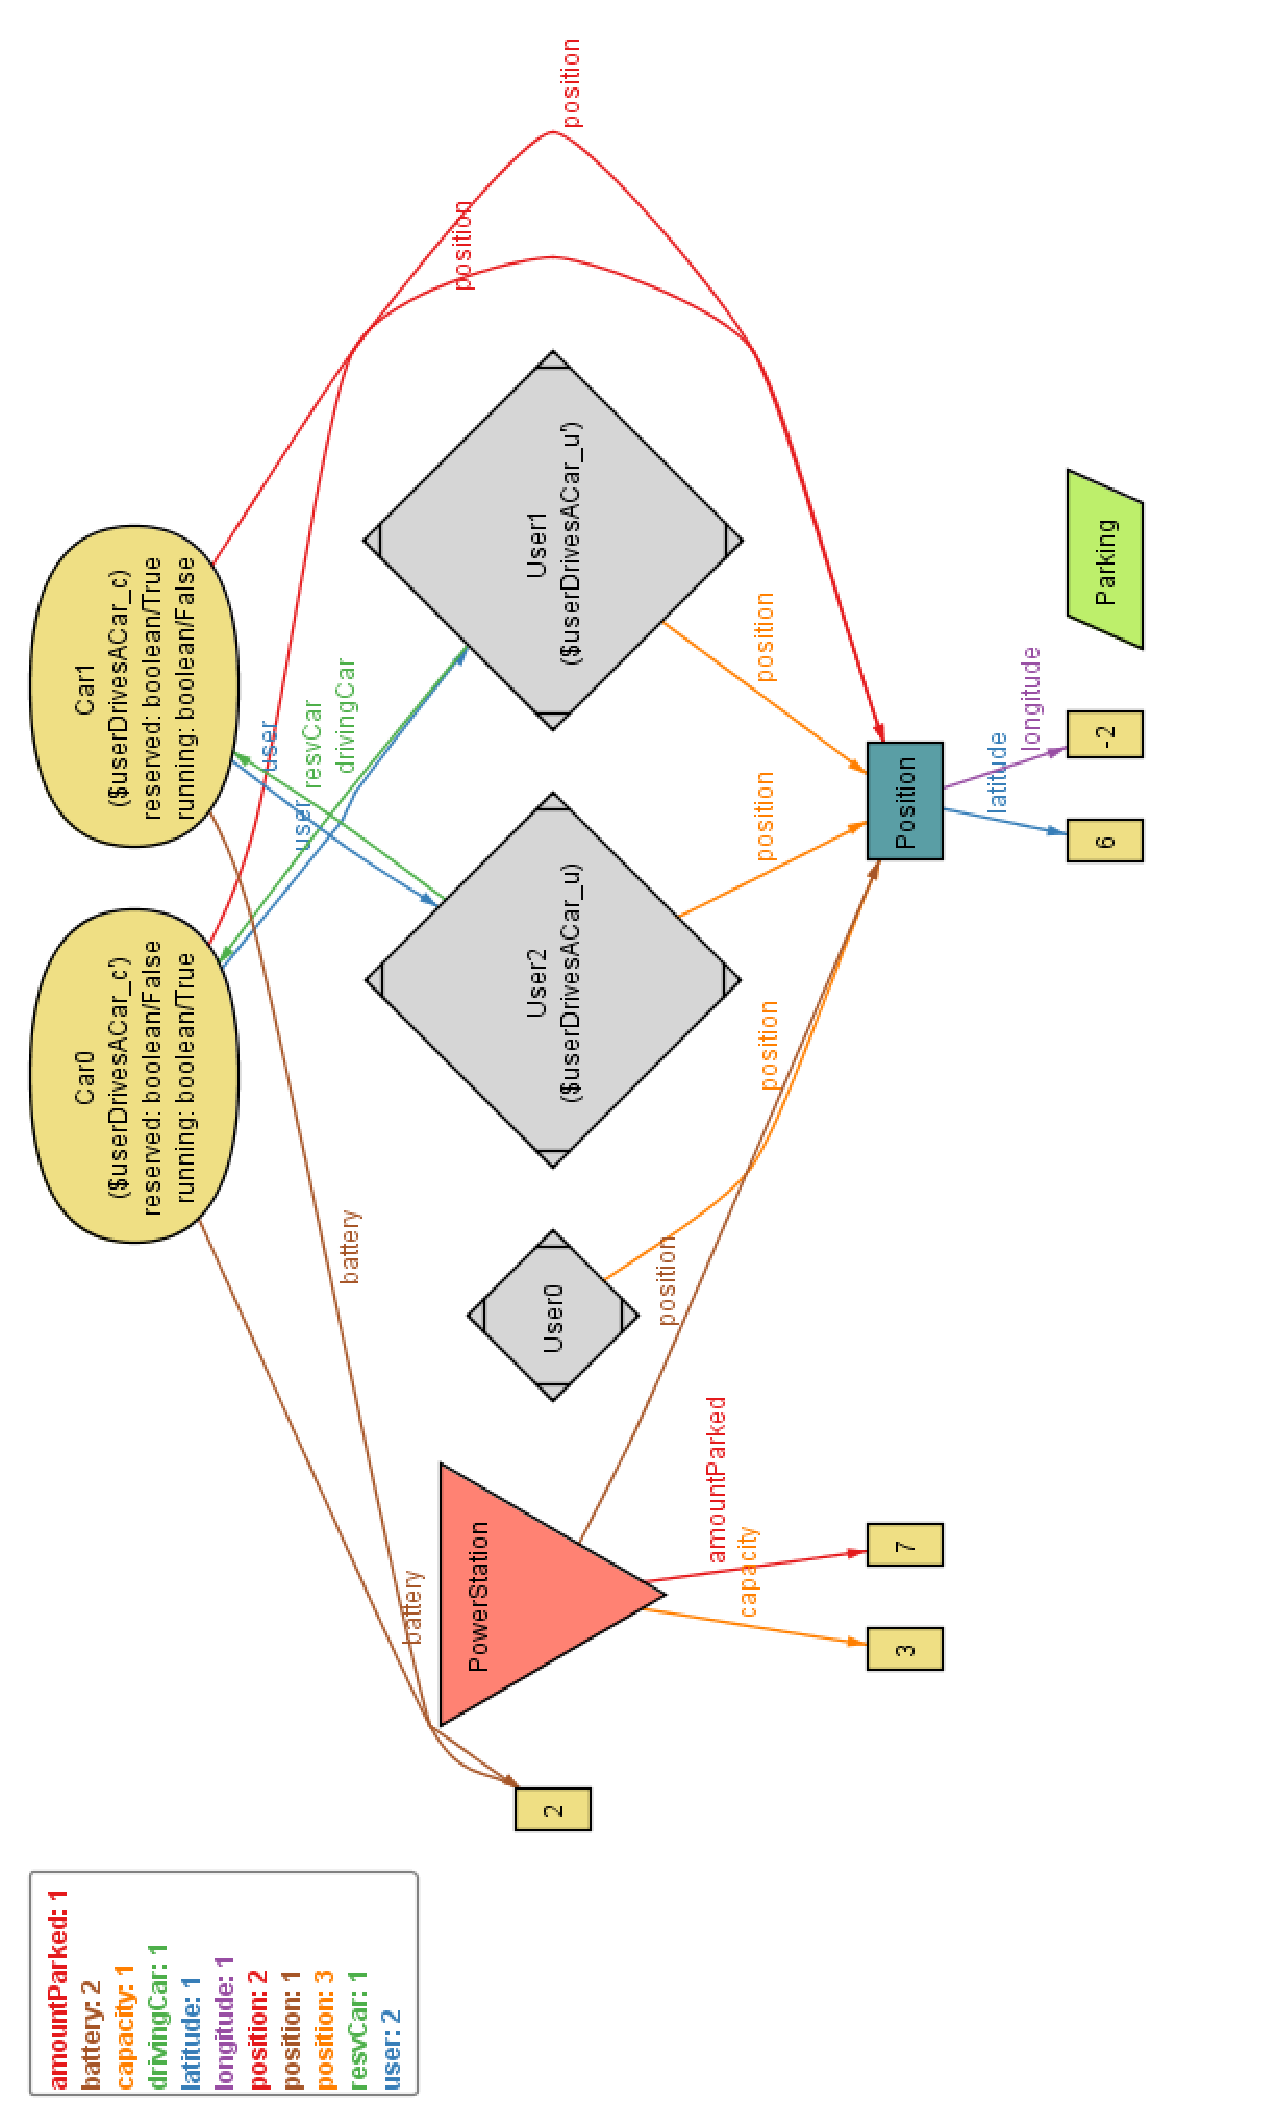
\includegraphics[height=15.2cm,keepaspectratio]{figures/world_generated_driving.eps}
	\caption{World generated for predicate \#1}
	\label{fig:world_generated_driving}
\end{figure}

\clearpage
\subsection{UserReservesACar}
\begin{figure}[h]
	\centering
	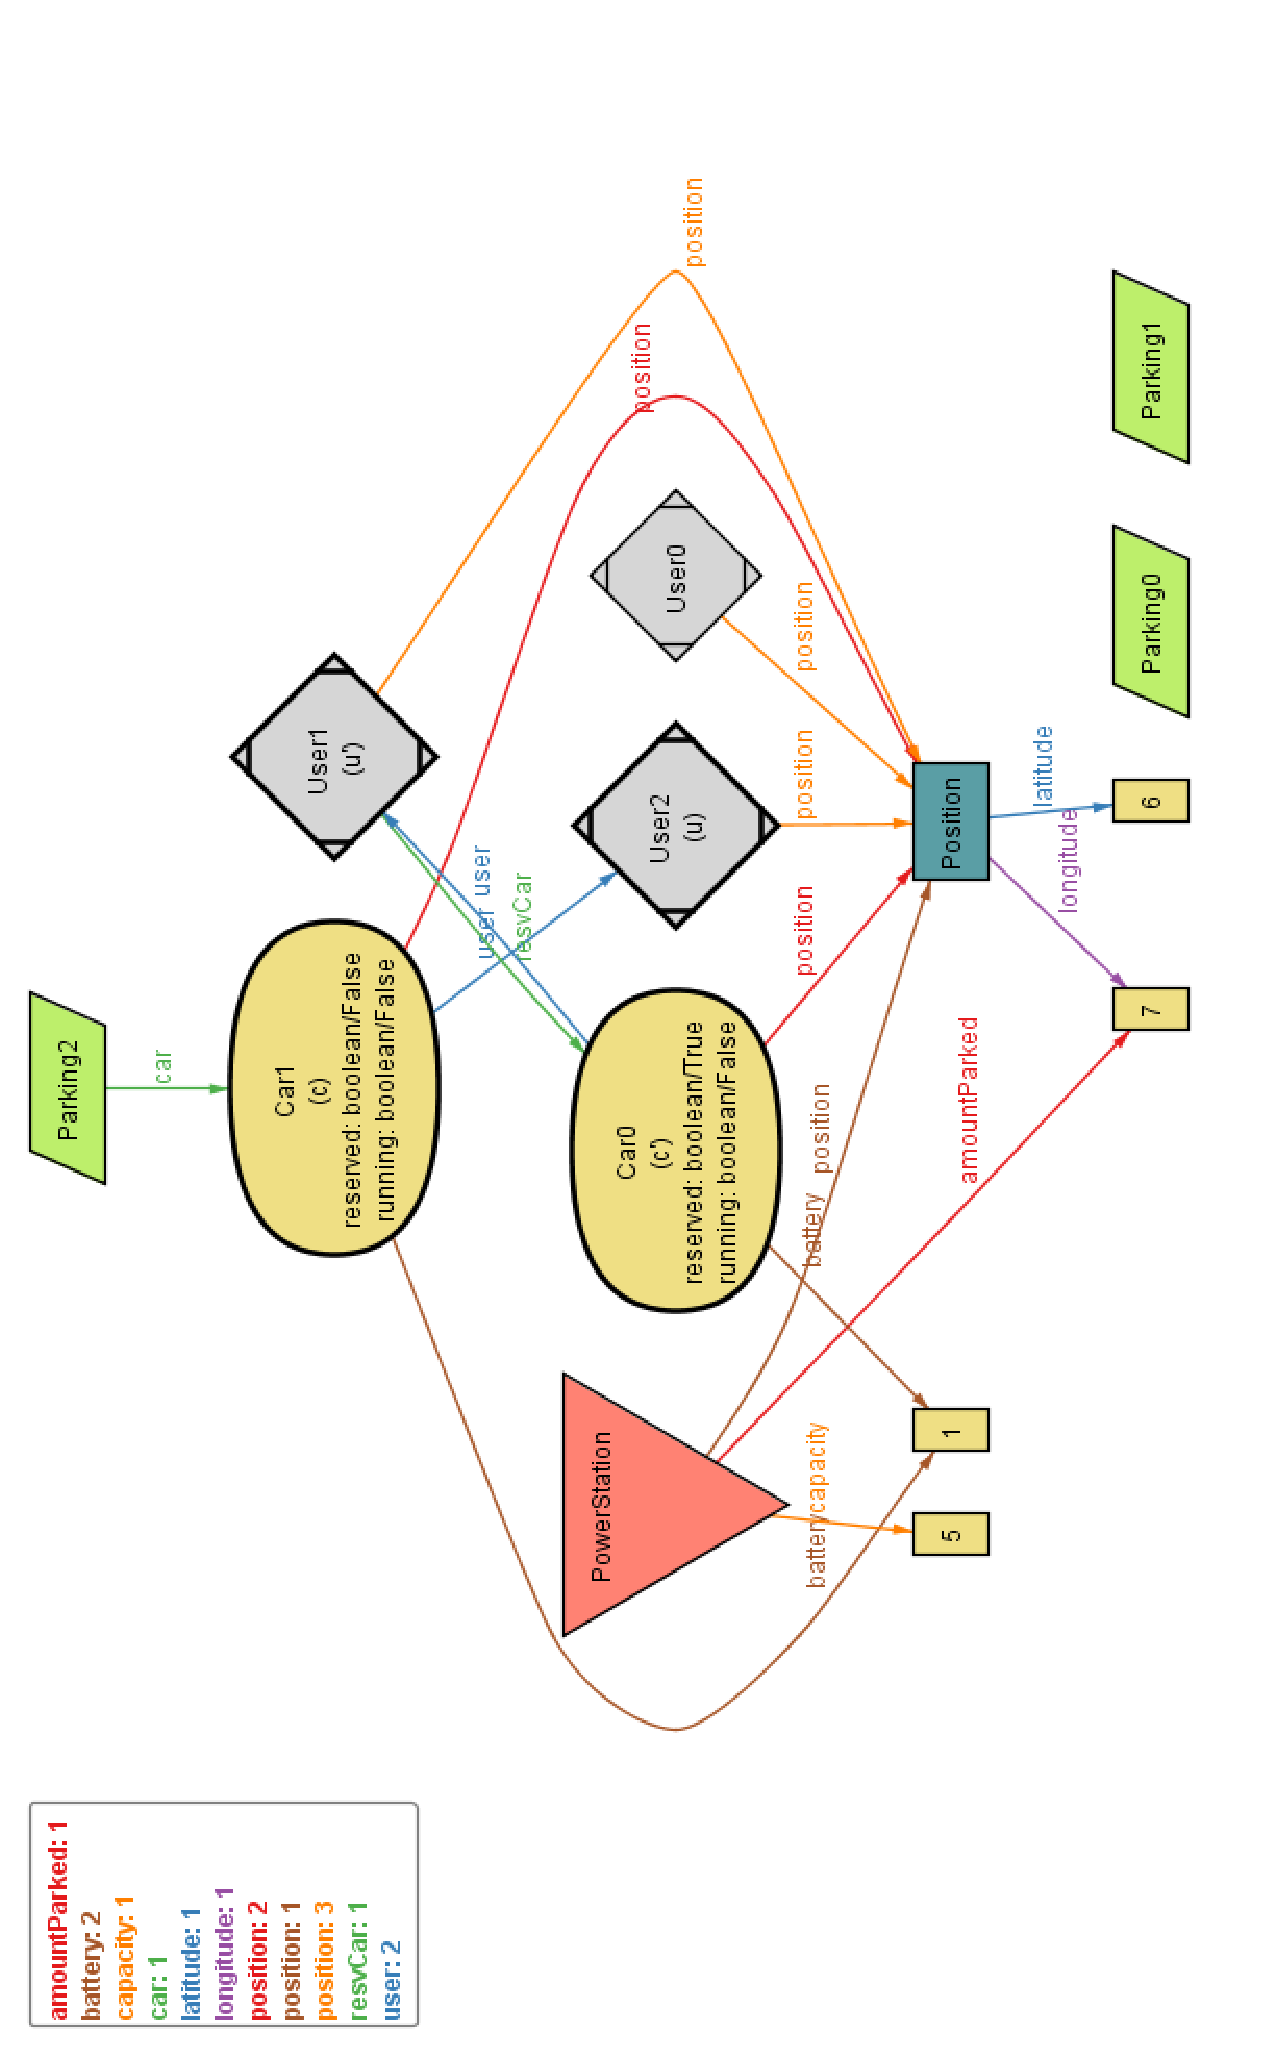
\includegraphics[height=15.2cm,keepaspectratio]{figures/world_generated_reservation.eps}
	\caption{World generated for predicate \#3}
	\label{fig:world_generated_reservation}
\end{figure}
